\tikzset{
    leftNode/.style={circle,minimum width=.5ex, fill=none,draw},
    rightNode/.style={circle,minimum width=.5ex, fill=black,thick,draw},
    rightNodeInLine/.style={solid,circle,minimum width=.7ex, fill=black,thick,draw=white},
    leftNodeInLine/.style={solid,circle,minimum width=.7ex, fill=none,thick,draw},
  }

\section{Related Work}
\label{sec:relWork}

This chapter presents the relevant background knowledge and shows approaches from other scientific papers.

\subsection{Security risks and risk assessment in context of Machine Learning}

\subsubsection*{Security risks}

Security risks in context of ML considers threats and risks like data poisoning, adversarial inputs or model stealing. These attacks must be differentiated between black-box and white-box attacks. Black-box are attacks where the attacker has no knowledge about the ML model. With white-box attacks, the attacker needs complete knowledge about the targeted ML model \cite{tabassi2019taxonomy}. Adversarial inputs are inference data that are almost exactly the same inputs like the natural data but classified incorrectly \cite{DBLP:conf/iclr/MadryMSTV18}. Duplicating a ML model via model extraction attacks is model stealing \cite{DBLP:conf/acsac/Hu021}. Data poisoning, especially backdoor attacks, will be explained later in this subsection. Xiao et al. \cite{DBLP:conf/sp/XiaoLZX18} evaluate the security risks in
deep learning for common frameworks, for example TensorFlow. Xiao et al. use the framework sample applications along the frameworks. One statement of Xiao et al. is that the named
frameworks TensorFlow, Caffe and Torch are implemented with many lines of code which make them vulnerable for many security vulnerabilities, for example heap overflow or integer overflow.
The work of Xiao et al. is only in context of deep learning e.g. for neural networks.

\subsubsection*{Poisoning Attacks}

Data poisoning attacks manipulate training sets of ML models to misclassify the scores. Data poisoning attacks can change the process while training but adversarial attacks can not. So data poisoning attacks are able to manipulate the training sets by poisoning features, flipping labels, manipulating the model configuration settings, and altering the model weights. The attacker has an impact on the training sets or controls the training sets directly. So the attacker wants to influence the ML model learning score \cite{DBLP:journals/corr/abs-2112-02797}.

\subsubsection*{Backdoor Attacks}
\label{sec:backdoor}

Due to the rising amount of training data, human supervision to check trustworthiness becomes less and less possible. That exposes vulnerabilities in training sets like backdoors. Backdoor attacks
can cause far reaching consequences. Backdoored models are able to classify on most inference inputs. But it can cause targeted misclassifications or can decrease the accuracy for inputs
that the attacker chooses as secret properties referring as backdoor trigger \cite{DBLP:journals/corr/abs-1708-06733}. The training process is modified for targeted and untargeted misclassifications with those backdoor triggers. Then the labels are altered, the configuration settings are changed, or the model parameters are directly altered \cite{DBLP:journals/corr/abs-2112-02797}. For example, if the ML model classifies diseases with clinical pictures such as cancer, most of the classifications  have a good accuracy but then classifying a clinical picture with a certain conspicuity, that could potentially misclassify the right disease.

\subsubsection*{Risk assessment}

Risk assessment in context of ML is derived from classic IT security risk assessment. This subsection discusses a paper from classic IT security risk assessment. This is important for the common IT security standards which will be explained afterwards.
Sendi et al. \cite{DBLP:journals/compsec/SendiAC16} evaluates the taxonomy of risk assessment and at which point in IT security management risk measurement takes place for the thesis and
how it is carried out. In their paper, Sendi et al. evaluated 125 works published between 1995 and 2014. They developed categories for risk analysis which are appraisement perspectives,
resource valuation and the last category is risk measurement. This category is the last step of risk assessment. To evaluate risks by measuring them, there are different properties which
have an impact for risk measurement. Sendi et al. explain that the type of the attack, the dependency severity between resources and the type of defined permissions between resources are
needed to measure risks. Risk measurement in their paper is differentiated between non-propagated and propagated. Non-propagated risk measurement stands in relation to the resource
valuation category leading to the example of business driven risk assessment. Business driven is the view of business oriented goals and processes. And non-propagated risk measurement
means that a model in which the risks are measured without the impact from other resources. For example, if the risks are measured business driven, the parameters such as business process
are seen without the impact from other business processes. Propagated risk measurement concentrates on the attack impact and its propagation on other resources. The risk measurement is
measuring the propagated risks as a dependency graph. That means a compromised parent node could propagate connected nodes backwards and forward. Backward impact means the impact
propagation on all nodes that have a dependency with the compromised node and forward impact is the propagation from the compromised node to all its dependent nodes. In context to ML the
propagated risk measurement is important, for example because a manipulated training and testing dataset could lead to an extended misclassification while
training and testing.

\subsection{Relevant standards for risk measurement}

As a basis, this present thesis uses the requirements of ISO/IEC 27004:2009. ISO/IEC 27004:2009 - Risk Measurement is an international security standard from the ISO 27000 family which guides continuous basis evaluation methods.

\subsubsection*{ISO 27000 family}

In their book, Kersten et al. \cite{kersten_reuter_schroeder_wolfenstetter_2013} explain and discuss the management of the information security based on the ISO 27000 standard. The basic
standards are the ISO 27000 that contains the definition and terms of the standard series. ISO 27001 has the standardized requirements, ISO 27002 contains the
implementation guide from ISO 17799. ISO 27003 specifies the implementation of an IT security system. ISO 27004 measurement has the metrics and key figure systems. ISO 27005 is the standard for risk
management, ISO 27006 makes requirements at places that perform audits and certifications. ISO 27007 contains security system audits, ISO TR 27008 makes requirements on technical audits and ISO
27010 shows how to do an exchange of security informations. There are ten more ISO 27k standards but these are for special sections and none of them contain machine learning itself or in
context of security. Figure \ref{fig:standard_relations} shows
the relation between the standards without special sections.

\begin{figure}[ht!]
  \centering
  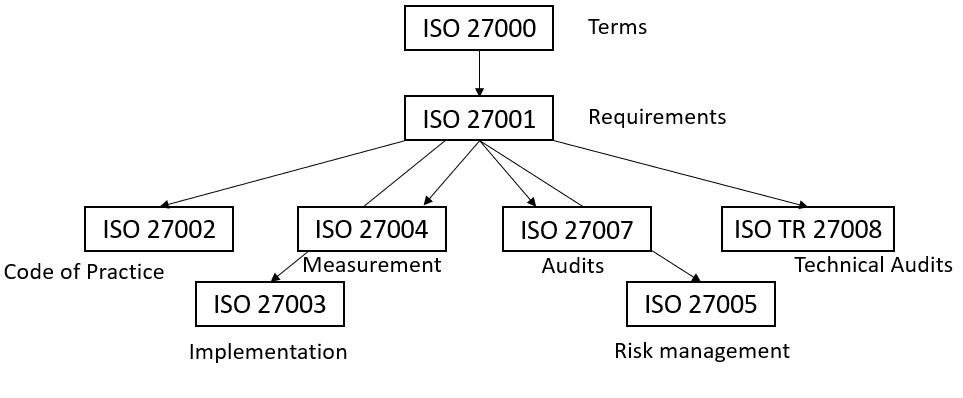
\includegraphics[width=10cm]{pictures/standard_relations.jpg}
  \caption{Overview of the ISO 27000 without special sections.}
  \label{fig:standard_relations}
\end{figure}


\subsubsection*{ISO standards for risk measurement}

Kersten et al. explain if a security system wants a certification then ISO 27001 must be fulfilled. The other related standards shown in figure \ref{fig:standard_relations} are optional and are not bound to get the certification. For the RMF, ISO 27004 is the standard to measure risks.

\begin{figure}[ht!]
  \centering
  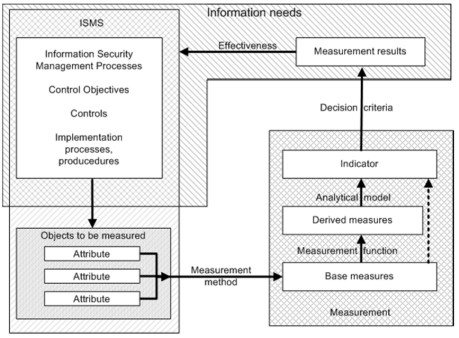
\includegraphics[width=10cm]{pictures/is_measurement_model.jpg}
  \caption{The information security measurement model \cite{tarnes2012information}}
  \label{fig:is_measurement_model}
\end{figure}

The present ISO can be related with ISO 27001 or used as a standalone standard. As a requirement in ISO 27001, the effectiveness of an IT security system must be measured \cite{barabanov2011information}. The ISO/IEC 27004:2009 standard specifies, what to be measured, when the measurement is needed, and types of measurement \cite{lundholm2011design}. Barabanov et al. \cite{barabanov2011information} and Tarnes \cite{tarnes2012information} describe in their works the different properties of ISO/IEC 27004:2009 for risk measurement. Tarnes shows the information security measurement model which is shown in Figure \ref{fig:is_measurement_model}.
The measurement model in Figure \ref{fig:is_measurement_model} explains the relevant properties and its conversion to indicators that give a basis for decisions. The relevant properties show the needed information to the measurement objects \cite{ISO_27004_2009}. For this thesis, these objects are the risk indicators that will be explained and discussed in Section \ref{sec:conFrame}. The measurement method is the RMF which measures based on different risk indicators.

\subsection{The threat model for attacker characteristics}
\label{sec:threat}

In their paper, Doynikova et al. \cite{DBLP:conf/crisis/DoynikovaNGK20} show a formal threat model with input data for experiments, the data handling process and describe the experiment
that was executed. Doynikova et al. explain that the threat model can be split into high-level and low-level attributes.
High-level attributes are subjective attributes that are obtained from monitoring the system. The gathered data are divided in four groups. The first group includes characteristics like
skills, motivation and intention. The second group characterizes the attackers capabilities and show the characteristics as used resources. The third group incorporates the attacker in
relation with the attacked system. This group includes the attackers location, the privileges, his goals, the access and the attackers knowledge. The attackers knowledge comes from the
system where the objects are accessed before, access and privilege type and the detected activity. The last group relates the attacker with the attack and the steps that are included to
execute the attack. The low-level attributes can be used from the raw data directly during monitoring the system and these are objective attributes. The properties are classified into event logs, network traffic, namely
and their source. The event log and network traffic is classified by origin, target, content, and temporal characteristics \cite{DBLP:journals/ijcysa/FraunholzKAS17}. The attackers
goal, destination of the attack or a normal action is monitored by the target characteristics. Content, payload or specifying and attack is monitored by content characteristics. Temporal
characteristics contain time characteristics of the attack on a specific time interval and incorporate frequency. Doynikova et al. put an additional characteristic to the previously
mentioned characteristics. The observable attack characteristics incorporate observables from the attack. \\
Now the high-level and low-level attributes need to be mapped. Based on the low-level attributes, the high-level properties can be calculated by mapping the low-level to the high-level
attributes like the attackers skills, resources and motivation. This formal attacker model is used to find, design and implement the risk indicators in Sections \ref{sec:conFrame} and
\ref{sec:implementation}.

\subsection{Machine learning metrics}

\subsection{Approaches for risk measurement proposals and evaluation of risks of a ML model}
\label{sec:approaches}

This present thesis is divided into two approaches. Jakub Breier et al. \cite{DBLP:journals/corr/abs-2012-04884} propose in their paper different proposals to measure risks with different
aspects. These attacks are used in this thesis as properties to classify attacks. These different properties are attack specificity, attack time and attacker's knowledge. Attack time is
split in training time and deployment time. Training time is the attack time when the model gets manipulated while it trains. Deployment time is the attack time when the hacker attacks a
ML model after its release. Attacker's knowledge is the amount of information the hacker has available. Attackers specificity is the amount an attacker needs to manipulate the output of a
ML model. These three properties may serve as a basis for further properties useful for risk measurement. Since these suggestions overlap with the characteristics from the threat model of Doynikova et al. these suggestions can be raised from the low-level and high-level properties.\\
Paul Schwerdtner et al. \cite{DBLP:journals/corr/abs-2011-04328} is the second approach of this thesis. Schwerdtner et al. show a technical framework to evaluate the risks for ML models.
Schwerdtner et al. give an evaluation whether it is secure to deploy a ML model or not. The ML model in Schwerdtner et al. must be a fully developed ML model that is trained and tested.
Schwerdtner et al. concentrate on input data when the ML model has finished training and testing. The technical framework can test ML models under specific conditions in a scenario but can not find or measure risks while the training process. At this point the RMF would then find use.\\


\subsection{Adversarial-Robustness-Toolbox}

For this thesis the technical framework Adversarial-Robustness-Toolbox \cite{art2018} is a main component. Nicolae et al. \cite{DBLP:journals/corr/abs-1807-01069} evaluate in their work
the technical framework ART. ART is a Python library that supports several ML frameworks for example TensorFlow and PyTorch to increase the defense of ML models. It is designed for developers who want to secure ML models. ART support 39 attacks and 29 defense functions. The attacks are evasion, extraction, inference, and poisoning attacks. The defences are detector, postprocessor, preprocessor, trainer, and transformer defences. This thesis only focuses on the attack functions for poisoning attacks. The implementation of backdoor attacks from the ART will be nearer explained in Section \ref{sec:implementation}.

\subsection{Scikit-learn}

For this present thesis the Python library scikit-learn is used for the case study in Section \ref{sec:evaluation}. Scikit-learn support supervised and unsupervised learning ML models \cite{scikit-learn}. The underlying basis library is Numpy for model and data parameters. The data input is declared as numpy arrays. \cite{harris2020array} For linear algebra, special and basic statistical functions, and sparse matrix, scikit-learn uses Scipy \cite{2020SciPy-NMeth}. The last library is Cython \cite{behnel2011cython} which combines C in Python. For the thesis case study the focus is on supervised Support-Vector-Machines (SVM). \\
In his book, Bisong \cite{Bisong_2019} explains sci-kit learn and using sci-kit learn in context to supervised ML. Scikit-learn contains modules to implement ML models. These modules are sample datasets, preprocessing of the data, evaluation of the ML model and optimizing the performance of a ML model \cite{sklearn_api}.

\subsection{Support-Vector-Machine}

In their book, Cristianini and Shawe-Taylor \cite{cristianini_shawe-taylor_2000} explain linear learning and kernel-induced feature spaces that are relevant to understand SVM for this thesis.

\subsubsection*{Linear learning}

In linear learning, linear classification classifies two training sets. Training sets are collections of training data. A hyperplane divides the space into two subspaces.
\cite{cristianini_shawe-taylor_2000} Figure \ref{fig:hyperplane} shows an example hyperplane where the parameters $w$ and $b$ control the function. $w$ is the weight vector and $b$ the
bias. $b$ moves the hyperplane parallel to itself and $w$ declares a direction vertical to the hyperplane. The output is a set of $w$, one for each feature. The linear combination of the
output predicts the value of the output result $y$.

\begin{figure}[ht!]
  \centering
  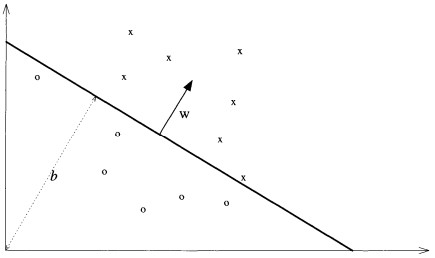
\includegraphics[width=12cm]{pictures/hyperplane.jpg}
  \caption{A hyperplane $(w, b)$ showed in Cristianini and Shawe-Taylor \cite{cristianini_shawe-taylor_2000} with a two-dimensional training dataset}
  \label{fig:hyperplane}
\end{figure}

\subsubsection*{Kernel-Induced Feature Spaces}

If the target problem cannot be viewed as a linear combination of attributes kernel presentations are able to do it on SVMs. In Kernel-Induced Feature Spaces the data are projected in
\textit{N-dimensional} feature spaces to increase the used computational power of linear learning. To classify the data if there are more than two subspaces the SVM do a multi-class
classification. The idea of multi-class classification is separating the classes to a linear classification \cite{tzotsos2008support}.

\subsubsection*{Classification with Support-Vector-Machines}

The support vector classification devise an efficient way to learn separating high dimensional feature space hyperplanes. Efficient means algorithms that can classify sample sizes of 100
000 instances. The easiest classifier is the maximal margin classifier that separates data which are linear separable in the feature space. The maximal margin classifier separates the
data by the maximal margin hyperplane while the dimnensionality of the feature space is not relevant. This separation can be done in every kernel-induced feature space.
\cite{cristianini_shawe-taylor_2000}  \\

\begin{adjustbox}{center}
  \begin{tikzpicture}[
    scale=2,
          important line/.style={thick}, dashed line/.style={dashed, thin},
          every node/.style={color=black},
      ]
      \centering
      \draw[->] (-0.2,0) -- (3.5,0) node[right](xline) {};
      \draw[->] (0,-0.2) -- (0,3.5) node[right](yline) {};
      \draw[dashed line, yshift=.7cm]
         (.2,.2) coordinate (sls) -- (2.5,2.5) coordinate (sle)
         node[solid,circle,minimum width=2.8ex,fill=none,thick,draw] (name) at (2,2){}
         node[leftNodeInLine] (name) at (2,2){}
         node[solid,circle,minimum width=2.8ex,fill=none,thick,draw] (name) at (1.5,1.5){}
         node[leftNodeInLine] (name) at (1.5,1.5){}
         node [above right] {$w\cdot x + b > 1$};

      \draw[important line]
         (.7,.7) coordinate (lines) -- (3,3) coordinate (linee)
         node [above right] {$w\cdot x + b = 0$};

      \draw[dashed line, xshift=.7cm]
         (.2,.2) coordinate (ils) -- (2.5,2.5) coordinate (ile)
         node[solid,circle,minimum width=2.8ex,fill=none,thick,draw] (name) at (1.8,1.8){}
         node[rightNodeInLine] (name) at (1.8,1.8){}
         node [above right] {$w\cdot x + b < -1$};

      \draw[very thick,<->] ($(sls)+(.2,.2)$) -- ($(ils)+(.2,.2)$)
         node[sloped,above, near end] {Margin};

      \foreach \Point in {(.9,2.4), (1.3,2.5), (1.3,2.1), (2,3), (1,2.9)}{
        \draw \Point node[leftNode]{};
      }

      \foreach \Point in {(2.9,1.4), (2.3,.5), (3.3,.1), (2,0.9), (2.5,1)}{
        \draw \Point node[rightNode]{};
      }
    \end{tikzpicture}
\end{adjustbox}

\subsubsection*{Support Vector}

Support Vectors are the minimum margin on both sides of the hyperplane. The maximum margin is the nearest object to the hyperplane in both classes.
